%=======================+=========================
%================  Online  ================
%=================================================

%------------------------------------------------------------------
\section[Online computing system]{Online computing system \label{sec:online}}

This section describes the \GX ~software and computing systems that are used for both data monitoring and transport to the tape system for permanent storage.

%------------------------------------------------------------------
\subsection{Monitoring \label{sec:onlinemonitoring}}

The Online Monitoring system (OMS) consists of multiple stages that provide for immediate monitoring of the data, as well as near-term monitoring ($\sim$hours after acquisition). The immediate monitoring is based on the \textit{RootSpy} system\cite{rootspy} written for use in \GX. Figure \ref{fig:online_monitoring_processes} shows a diagram of the processes involved in the RootSpy system and how they are coupled to the DAQ system. The Event Transfer (ET) is part of the CODA DAQ system\cite{coda} and is used to extract a copy of a portion of the data stream without interfering with the DAQ itself. The monitoring system itself utilizes a secondary ET in order to minimize connections to the RAID server that is running the Event Recorder process.

\begin{figure}[tbp]
\begin{center}
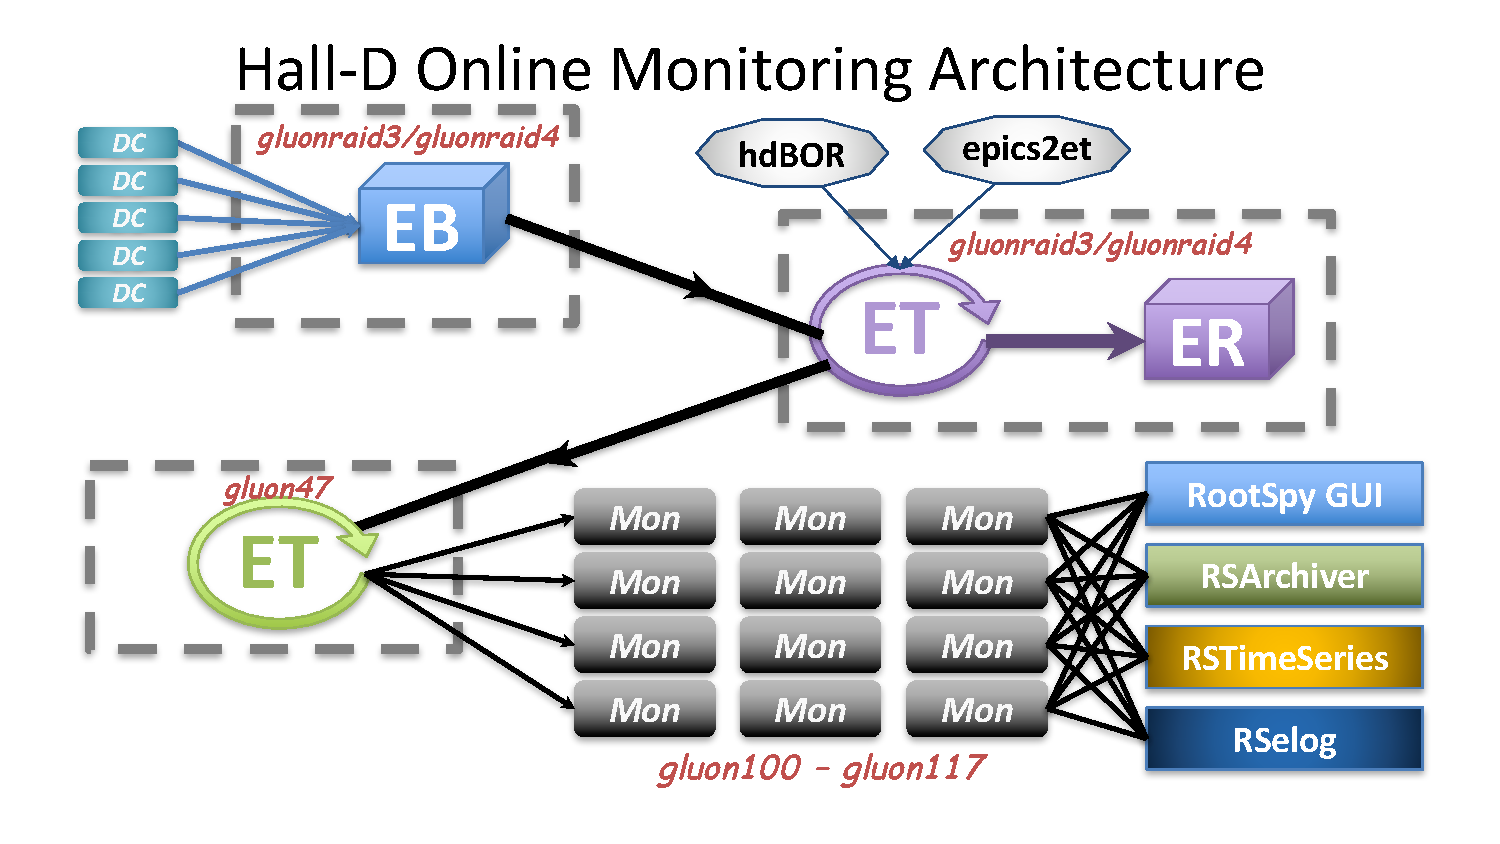
\includegraphics[width=0.99\textwidth, clip,trim=1.5cm 0.9cm 1.7cm 0.8cm]{figures/online_monitoring_processes.pdf}
\caption{\label{fig:online_monitoring_processes}Diagram of the various processes distributed across several computers in the counting house that make up the online monitoring system. DC, EB, and ER represent the Data Concentrator, Event Builder, and Event Recorder processes respectively in the CODA DAQ system.}   
\end{center}  
\end{figure}

RootSpy was developed at JLab for \GX, though its design is not \GX ~specific. The system is run on a small farm of computers\footnote{The online monitoring farm consists of eight 2012 era Intel x86\_64 computers with 16 cores+16ht plus six 2016 era Intel x86\_64 computers with 36 cores + 36ht. The monitoring farm uses 40 Gbps (QDR) and 56 Gbps(FDR) IB for the primary interconnect. Note that the DAQ system uses a separate 40 Gbps ethernet network that is independent of the farm.} in the counting house, each processing a small part of the data stream. In total, about 10\% of the data is processed for the low level occupancy plots while roughly 2\% is fully reconstructed for higher level plots. The CODA ET software system is used to distribute the data among the farm computers. Each farm node generates histograms which RootSpy gathers and combines before displaying them to shift workers in a GUI.
%Figure \ref{fig:online_monitoring_rootspy} shows a screen capture of the main RootSpy GUI window along with a window displaying the reference plot for the currently displayed image.
Plots are displayed via a set of ROOT macros, each responsible for drawing a single page. Most macros divide the page into multiple sections so that multiple plots can be displayed on a single page. Figure \ref{fig:online_monitoring_PID} shows an example of a high level monitoring plot where four invariant mass distributions are shown with fits. Values extracted from the fits are printed on the plots for easy quantitative comparison to the reference plot. 

Shift workers are presented with a live plot alongside a reference plot by which to compare. Shift workers may assign a live plot as the new reference using a button on the RootSpy GUI. Relevant experts for the given plot are notified via e-mail when a new reference is made thus, providing for expert oversight of the reference plots.

ROOT macros are passed into the RootSpy GUI using the same xMsg\cite{xmsg} publish subscribe messaging system used to transport histogram objects. The macros are compiled into plugins as C++ strings by the build system. The build system recognizes ROOT macro files in the plugin source directory (via the .C suffix) and automatically generates C++ code that contains the macro and code to register it with the RootSpy system. This is done to ensure that a macro is always in sync with the histograms it displays since the former is linked in the same binary as the routines that produce the latter.

\begin{figure}[tbp]
\begin{center}
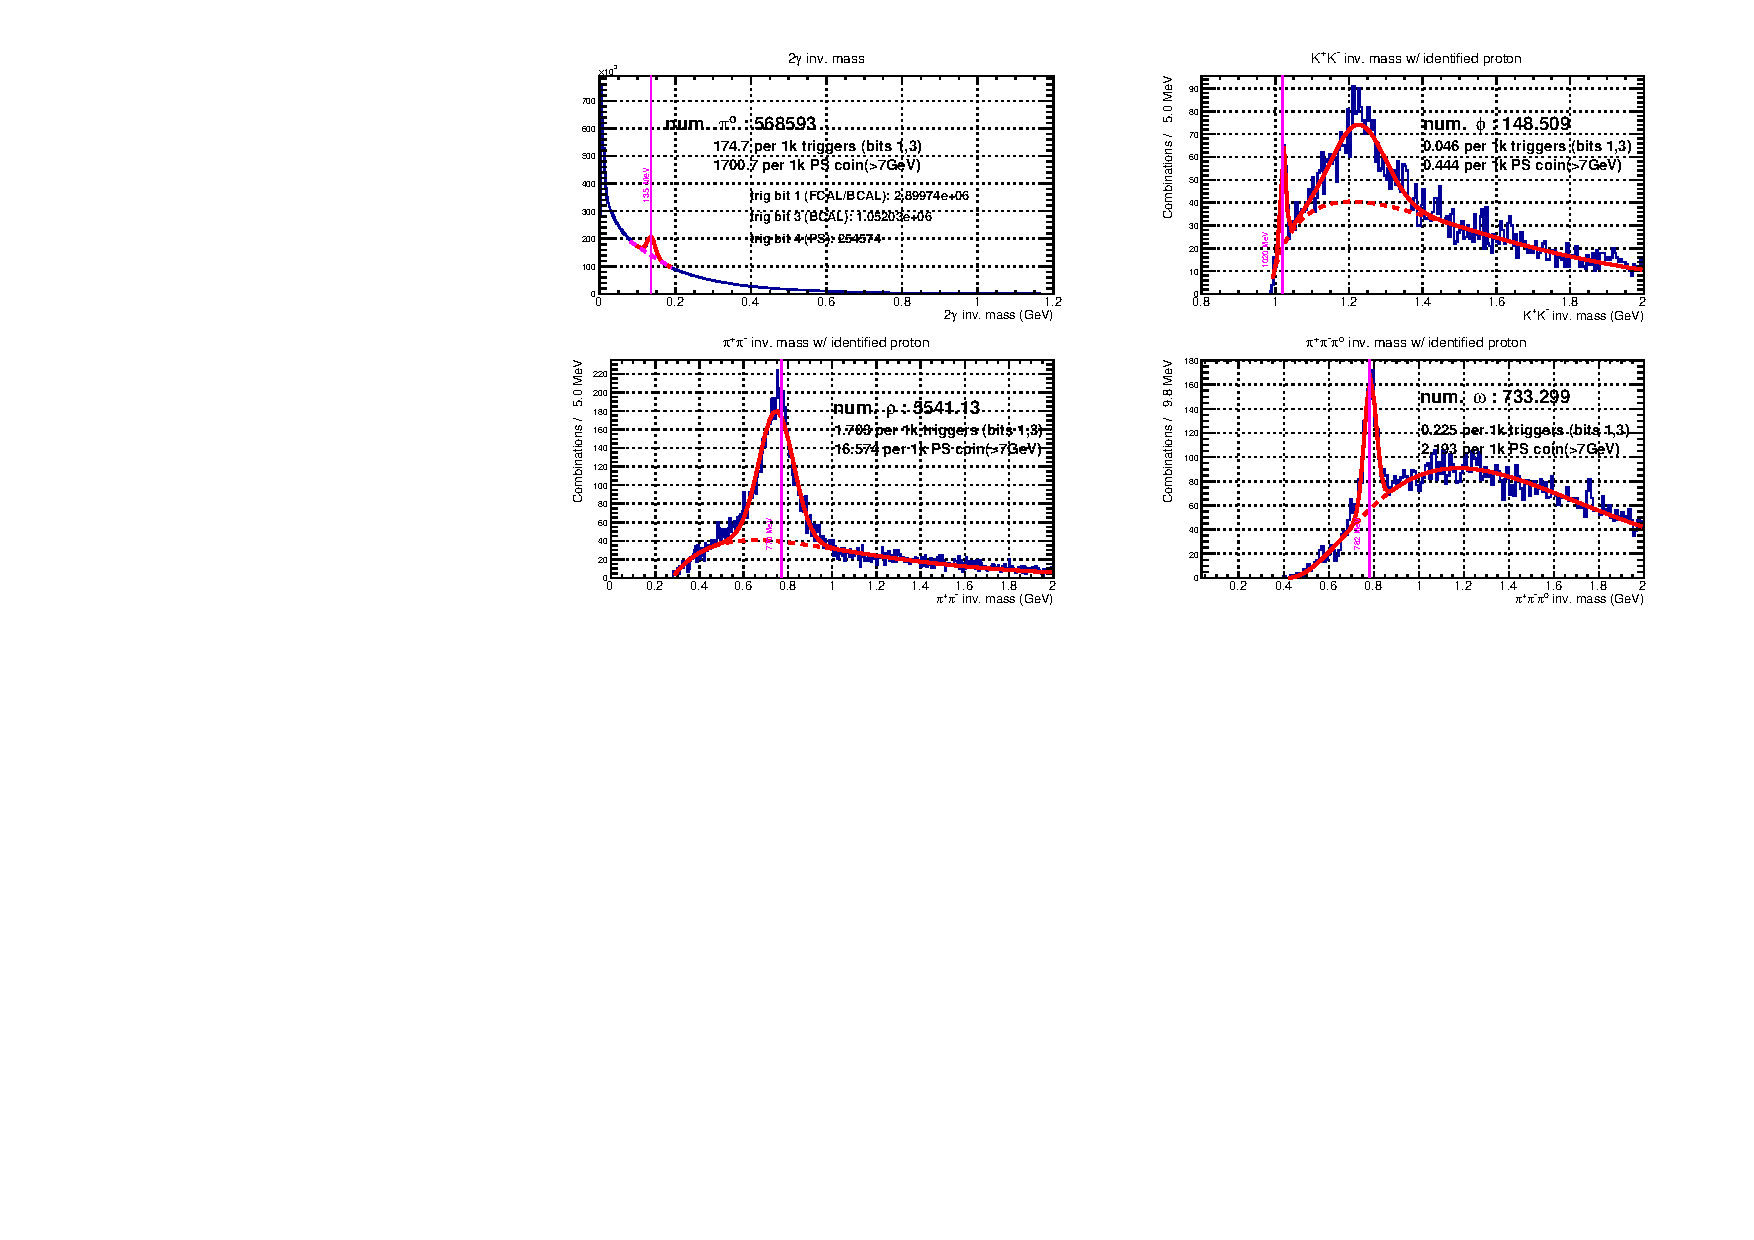
\includegraphics[width=0.99\textwidth, clip,trim=0.6cm 0.0cm 1.1cm 0.0cm]{figures/online_monitoring_PID.pdf}
\caption{\label{fig:online_monitoring_PID}Invariant mass distributions showing $\pi^\circ$, $\omega$, $\rho$, and $\phi$ particles. These plots were generated online in about 1hr 40min by looking at roughly 2\% of the data stream.}   
\end{center}  
\end{figure}

In addition to the RootSpy GUI, several other client programs exist that consume the histograms being produced by the RootSpy system. One of these is the RSTimeSeries program. This program periodically runs a subset of macros that contain special calls to insert data into an InfluxDB time series database. This provides a web-accessible strip chart of detector hit rates and reconstructed quantities (e.g. number of $\rho$'s per 1k triggers). The RSArchiver program gathers summed histograms and periodically writes them to a ROOT file for permanent archival. The archive file is later used to generate a set of image files that are displayed in the Plot Browser\footnote{https://halldweb.jlab.org/data\_monitoring/Plot\_Browser.html.} website. Plot Browser allows for easy comparison of plots for different runs as well as with similar plots produced during offline analysis. The first five files (100GB) of each run are automatically pinned to disk in the JLab Computing Center after being transported there for permanent tape storage. Jobs are automatically submitted for these files to the JLab SciComp farm to perform full reconstruction. The results of this are displayed in Plot Browser under the title ``Incoming Data.''


%------------------------------------------------------------------
\subsection{Data Transport and Storage \label{sec:onlineprocessing}}

\GX ~Phase I generated production data at rates up to 650MB/s. The data was temporarily stored on large RAID-6 disk arrays and then copied to an LT0 tape system for long term storage. Two RAID servers, each with four partitions were used in the Hall-D counting house. The partition being written to was rotated between runs through the use of symlinks. This helped to minimize head thrashing on disks by only reading from the partitions not currently being written to. Partitions were kept at approximately 80\% full and older files deleted only as needed to maintain this. This was to allow the monitoring farm easy access to the files for times when the beam was down. An additional copy of the first 3 files ($\sim1.5\%$) of each run was made to a smaller RAID disk so that an easily accessible sample of each run could be maintained in the counting house.

The data volumes stored to tape are shown in table \ref{tab:online_data_volumes} in units of petabytes(PB). Lines marked ``actual'' are values taken from the tape storage system. Lines marked ``model'' come from the \GX ~computing model\cite{gx3821}.

\begin{table}[]
    \centering
    \begin{tabular}{|l|c|c|c|c|c|}
    \hline
                           & \textbf{2016}  & \textbf{2017}  & \textbf{2018} \\
    \hline
    actual (raw data only) & 0.624 & 0.914 & 3.107 \\
    \hline
     model (raw data only) &       & 0.863 & 3.172 \\
    \hline
    \hline
    actual (production)    & 0.55  & 1.256 & 1.206 \\
    \hline
     model (production)    &       & 0.607 & 3.084 \\
    \hline
    \end{tabular}
    \caption{\GX ~Data volumes by year. All values are in petabytes(PB). Most years include two run periods. The lines marked \textit{model} are calculated from the \GX ~Computing Model\cite{gx3821}. ``raw data only'' represents data generated by the DAQ system (not including the backup copy). ``production'' represents all data derived from that (reconstructed values and ROOT trees). }
    \label{tab:online_data_volumes}
\end{table}

